% Bar Chart - Biomasse Bruttostromerzeugung 2019

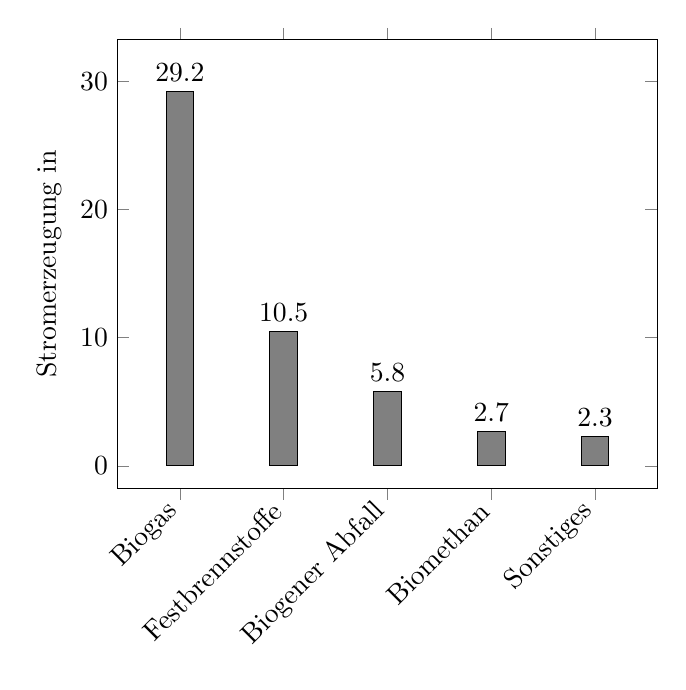
\begin{tikzpicture}
	\begin{axis}[
	ybar,
	enlargelimits=0.15,											% äüßerste bar plots nicht am Limit der x-Achse
	ylabel={Stromerzeugung in \si{\twh}},
	symbolic x coords={Biogas,
		Festbrennstoffe,
		Biogener Abfall,
		Biomethan,
		Sonstiges 
	},
	xtick=data,
	nodes near coords,											% Zahlen auf den bar plots
	nodes near coords align={vertical},
	x tick label style={rotate=45,anchor=east},
	]
	\addplot[black,fill=black!50!white] coordinates {
		(Biogas,29.2) (Festbrennstoffe,10.5) (Biogener Abfall,5.8)
		(Biomethan,2.7) (Sonstiges,2.3)
	};
	\end{axis}
\end{tikzpicture}